\subsection{Results for Trajectories Estimated Using $x$ and $y$ Offset}
%\label{subsec:no_abs_results}
%\vspace{10pt}

Figure~\ref{fig:best_RMSE_traj_val} contains the average RMSE across $k$-fold testing datasets using different trajectory estimation methods, validation datasets for all trajectories estimated in nested $k$-fold cross-validation by different trajectory estimation methods, RNN models, and forecasting times.

\begin{figure}[!ht]
	\centering
	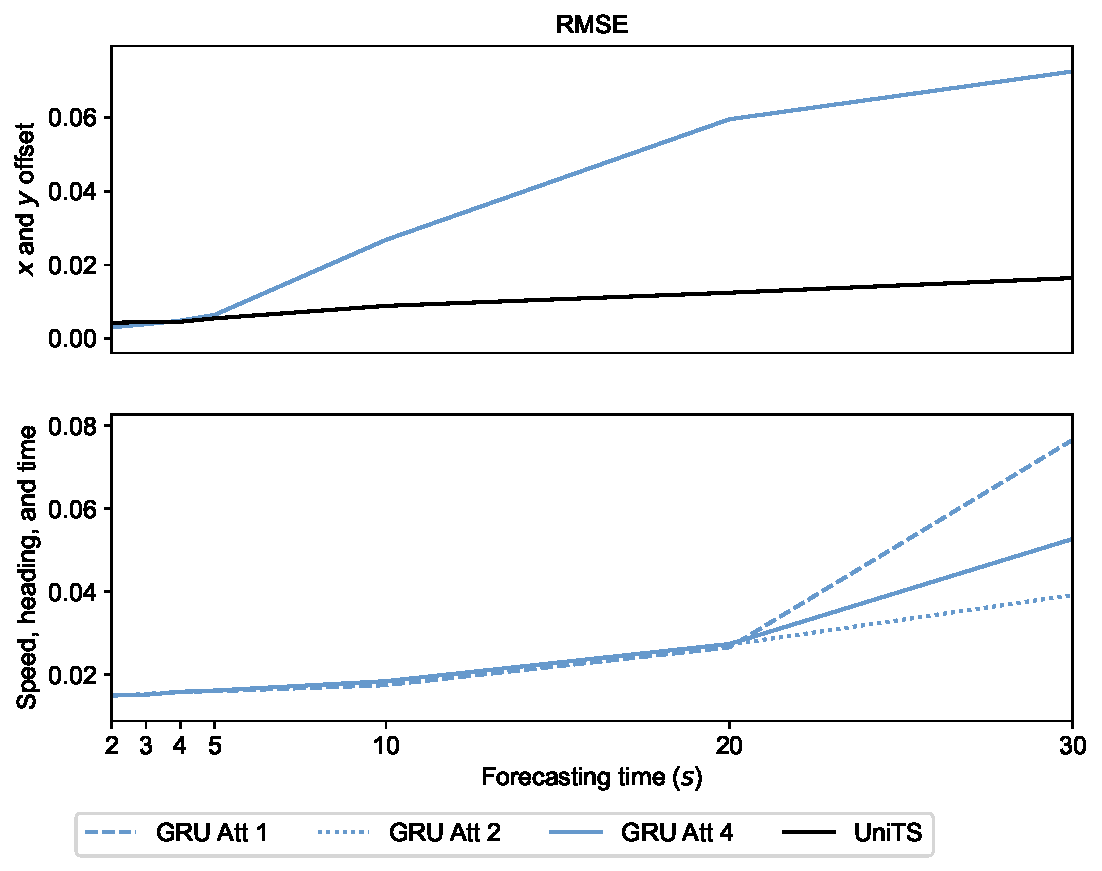
\includegraphics[width = 0.99 \linewidth]{best_RMSE_traj_val.pdf}
	\caption{The average RMSE across $k$-fold testing datasets using different trajectory estimation methods, validation datasets for all trajectories estimated in nested $k$-fold cross-validation by different trajectory estimation methods, RNN models, and forecasting times.}
	\label{fig:best_RMSE_traj_val}
\end{figure}

The average RMSE ($\times 10^{-3}$), with standard deviation in brackets, across $k$-fold validation datasets for the trajectories in the $k$-fold testing datasets estimated using $x$ and $y$ offset, different RNN models, and forecasting times is listed in Table~\ref{tab:best_no_abs_RMSE}.

\begin{table}[!ht]
	\centering
	\resizebox{\linewidth}{!}{
		\begin{tabular}{|c|c|c|c|c|c|c|c|}
			\hline
			Model & $2$ $s$ & $3$ $s$ & $4$ $s$ & $5$ $s$ & $10$ $s$ & $20$ $s$ & $30$ $s$ \\ \hline
			\multirow{2}{*}{GRU Att 4} & $\mathbf{3.05}$ & $\mathbf{3.86}$ & $4.86$ & $6.4$ & $26.8$ & $59.52$ & $72.49$ \\
			 & \textbf{(}$\mathbf{0.49}$\textbf{)} & \textbf{(}$\mathbf{0.51}$\textbf{)} & ($0.52$) & ($0.85$) & ($6.96$) & ($9.83$) & ($19.4$) \\ \hline
			\multirow{2}{*}{UniTS} & $4.26$ & $4.47$ & $\mathbf{4.54}$ & $\mathbf{5.47}$ & $\mathbf{8.86}$ & $\mathbf{12.43}$ & $\mathbf{16.41}$ \\
			 & ($3.51$) & ($2.91$) & \textbf{(}$\mathbf{0.66}$\textbf{)} & \textbf{(}$\mathbf{0.97}$\textbf{)} & \textbf{(}$\mathbf{1.37}$\textbf{)} & \textbf{(}$\mathbf{1.55}$\textbf{)} & \textbf{(}$\mathbf{2.47}$\textbf{)} \\ \hline
		\end{tabular}
	}
	\caption{The average RMSE ($\times 10^{-3}$), with standard deviation in brackets, across $k$-fold validation datasets for the trajectories in the $k$-fold testing datasets estimated using $x$ and $y$ offset, different RNN models, and forecasting times.}
	\label{tab:best_no_abs_RMSE}
\end{table}

The GRU Att 4 model achieved the lowest RMSE for trajectories estimated using $x$ and $y$ offset, and a forecasting time of $2$, and $3$ $s$ with average values and standard deviation (in brackets) that equal $3.05 \times 10^{-3}$ $\degree$ ($0.49 \times 10^{-3}$ $\degree$), and $3.86 \times 10^{-3}$ $\degree$ ($0.51 \times 10^{-3}$ $\degree$) respectively.

The UniTS model achieved the lowest RMSE for trajectories estimated using $x$ and $y$ offset, and a forecasting time of $4$, $5$, $10$, $20$, and $30$ $s$ with average values and standard deviation (in brackets) that equal $4.54 \times 10^{-3}$ $\degree$ ($0.66 \times 10^{-3}$ $\degree$), $5.47 \times 10^{-3}$ $\degree$ ($0.97 \times 10^{-3}$ $\degree$), $8.86 \times 10^{-3}$ $\degree$ ($1.37 \times 10^{-3}$ $\degree$), $12.43 \times 10^{-3}$ $\degree$ ($1.55 \times 10^{-3}$ $\degree$), and $16.41 \times 10^{-3}$ $\degree$ ($2.47 \times 10^{-3}$ $\degree$) respectively.

